\graphicspath{{./figures}}

\section{Ground Station Antenna}

The initial helical antenna build is shown in Figure \ref{fig:gsAntennaOriginal}. 2.5 mm stranded copper wire was used due to its flexibility and availability. A cardboad ground plane wrapped in aluminium foil was used due to its lightweight nature. Further, a strip of harder aluminium tin was taped to the wire for the matching strip. Initially, the strip was over-sized, and more turns than necessary were used. A female panel-mounted SMA connector was mounted using bolts, and the antenna wire was soldered to the protruding pin.

The coiled wire is mechanically supported by a central PVC pipe and wooden dowels. Markings on the pipe were used to dimension the antenna. The materials were sized to provide stability, but not exceed the maximum torque limitations of the motors. The final antenna weight was measured at 344 g, giving a worst-case mass-distance product of $\SI{344}{g} \times \frac{\SI{45}{cm}}{2} \approx \SI{0.08}{kg \cdot m}$, which is under the maximum of $\SI{0.2}{kg \cdot m}$.

After initial testing, the matching strip was cut to size, a circular trapezoidal cut-out was made to support a lower elevation angle, and the number of turns was set to $n=4$. The system was eventually mounted onto a tripod, and a final photo of the full ground station out in the field is shown in Figure \ref{fig:gsTripod}.

\begin{figure}[!htb]
  \centering
  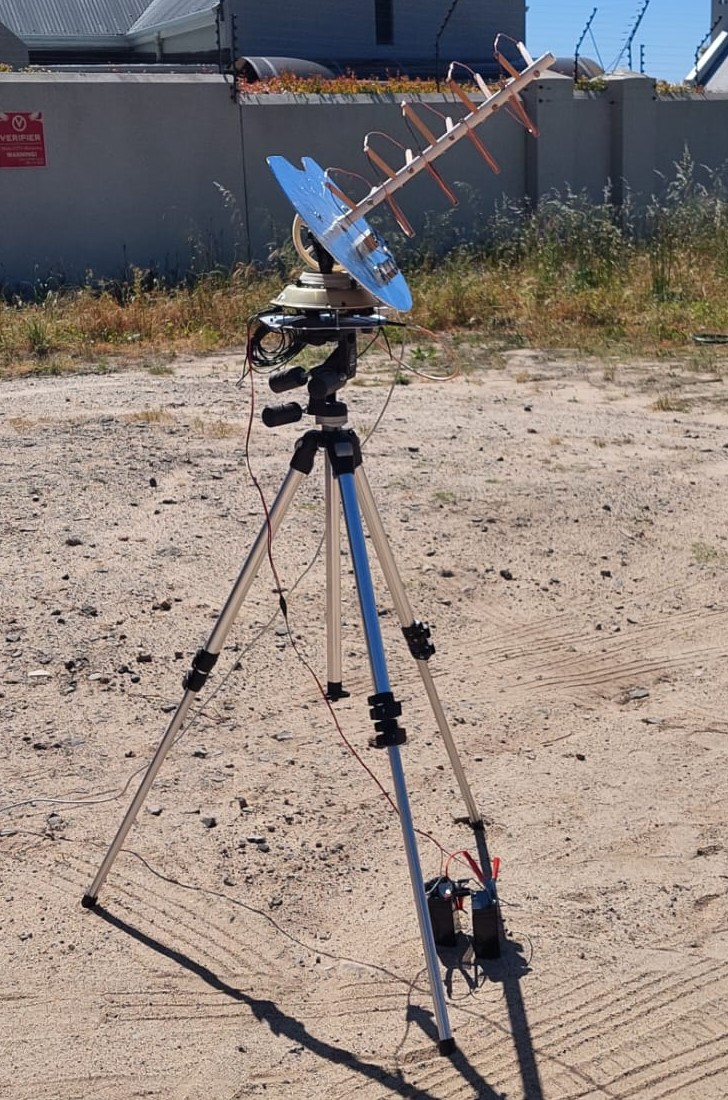
\includegraphics[width=0.5\textwidth]{gsTripod}
  \caption{Ground Station Mounted on Tripod}
  \label{fig:gsTripod}
\end{figure}